% The first command in your LaTeX source must be the \documentclass command.
\documentclass[acmlarge,screen,dvipsnames]{acmart}
%usepackage{color}
\usepackage{amsmath}
\usepackage{pseudocode}
\usepackage[ruled]{algorithm2e}
\usepackage{algorithmicx}
\usepackage{subcaption}
\usepackage{natbib}
%\usepackage{afterpage}  % for float-page placement trick
\usepackage{placeins}
\usepackage{gensymb}
\usepackage{amssymb}
\input widebar

\usepackage[normalem]{ulem}  % for strike-through (\sout)

\input twmacros
%
% defining the \BibTeX command - from Oren Patashnik's original BibTeX documentation.
\def\BibTeX{{\rm B\kern-.05em{\sc i\kern-.025em b}\kern-.08emT\kern-.1667em\lower.7ex\hbox{E}\kern-.125emX}}
 

\setcopyright{acmcopyright}
\acmJournal{JOCCH}
\acmYear{2020} \acmVolume{13} \acmNumber{1} \acmArticle{1} \acmMonth{1} \acmPrice{15.00}\acmDOI{10.1145/3351343}



% \usepackage{balance}
%
% Rights management information. 
% This information is sent to you when you complete the rights form.
% These commands have SAMPLE values in them; it is your responsibility as an author to replace
% the commands and values with those provided to you when you complete the rights form.
%
% These commands are for a PROCEEDINGS abstract or paper.
%\copyrightyear{2018}
%\acmYear{2018}
%\setcopyright{acmlicensed}
%\acmConference[Woodstock '18]{Woodstock '18: ACM Symposium on Neural Gaze Detection}{June 03--05, 2018}{Woodstock, NY}
%\acmBooktitle{Woodstock '18: ACM Symposium on Neural Gaze Detection, June 03--05, 2018, Woodstock, NY}
%\acmPrice{15.00}
%\acmDOI{10.1145/1122445.1122456}
%\acmISBN{978-1-4503-9999-9/18/06}

%
% These commands are for a JOURNAL article.

% \setcopyright{acmcopyright}
% \acmJournal{JOCCH}
% \acmYear{2020} \acmVolume{13} \acmNumber{1} \acmArticle{1} \acmMonth{1} \acmPrice{15.00}\acmDOI{10.1145/3351343}

%
% Submission ID. 
% Use this when submitting an article to a sponsored event. You'll receive a unique submission ID from the organizers
% of the event, and this ID should be used as the parameter to this command.
%\acmSubmissionID{123-A56-BU3}

%
% The majority of ACM publications use numbered citations and references. If you are preparing content for an event
% sponsored by ACM SIGGRAPH, you must use the "author year" style of citations and references. Uncommenting
% the next command will enable that style.
%\citestyle{acmauthoryear}

%
% end of the preamble, start of the body of the document source.
\begin{document}

%
% The "title" command has an optional parameter, allowing the author to define a "short title" to be used in page headers.


\title[Creative Experiences for engaging communities with cultural heritage]%
      {Creative Experiences for Engaging Communities with Cultural Heritage through Place-Based Narratives}
%
% The "author" command and its associated commands are used to define the authors and their affiliations.
% Of note is the shared affiliation of the first two authors, and the "authornote" and "authornotemark" commands
% used to denote shared contribution to the research.
% \author{Karina Rodriguez Echavarria}
% \email{K.Rodriguez@brighton.ac.uk}
% \orcid{0000-0002-8679-1602}
% \affiliation{%
%   \institution{Centre for Secure, Intelligent and Usable Systems, University of Brighton}
%   \city{Brighton}
%   \country{United Kingdom}
% }

% \author{Myrsini Samaroudi}
% \affiliation{%
%   \institution{Centre for Secure, Intelligent and Usable Systems, University of Brighton}
%   \city{Brighton}
%   \country{United Kingdom}
%   }

% \author{Tim Weyrich}
% \affiliation{%
%   \institution{Department of Computer Science, University College London}
%   \city{London}
%   \country{United Kingdom}
% }

%
% By default, the full list of authors will be used in the page headers. Often, this list is too long, and will overlap
% other information printed in the page headers. This command allows the author to define a more concise list
% of authors' names for this purpose.
\renewcommand{\shortauthors}{K. Rodriguez, et al.}

%
% A "teaser" image appears between the author and affiliation information and the body 
% of the document, and typically spans the page. 
\begin{teaserfigure}
\centering
 %  \subcaptionbox{Physical creative artwork created by children in the community\label{step1}}
 % {
 % 
 \includegraphics[width=.45\linewidth]{images/mapalone}
 % }
 % \subcaptionbox{Generated Augumented Reality Map with embedded digital elements of the artwork\label{step2}}{
 \includegraphics[width=.40\linewidth]{images/screenshoot}
 % }
 % \\[0.5\baselineskip]
  \caption{Artwork and Augmented Reality (AR) Map
with embedded creative narratives of the communities' cultural environment 
for dissemination to a wider audience\vspace*{0.5\baselineskip}}
  \label{fig:teaser}
\end{teaserfigure}


%-------------------------------------------------------------------------
\begin{abstract} 
This research explores technologically advanced means to enhance audiences' connection with cultural heritage assets through participatory creative methods which particularly reinforce young people's sense of identity and well-being, during sensitive ``transitional'' periods of their lives. Hence, the research investigates how communities can
meaningfully connect with cultural heritage through creative and digital
experiences, while aiming at lowering the entry barriers to increase audiences' participation.
For this, the research deploys creative and narrative or story-based approaches to illuminate different viewpoints and interpretations of cultural heritage within communities. The contribution of the paper is twofold, as it includes a novel approach for developing and re-telling communities' narratives linked to people, objects, sites and events in the urban landscape. At the same time, it proposes a workflow to communicate these narratives through \emph{Augmented
Reality (AR) Maps}. These are physical maps with augmented digital narratives, delivered through \emph{Immersive Web} technology. This concept is
proposed as a means to document and disseminate the narratives in a way that enhances the public understanding and appreciation of objects and sites. The approach was initially piloted with a class of 32 children in a local primary school in Brighton and Hove (UK) in order to understand its suitability for community engagement, targeting young audiences. Currently, the project has been expanded to five more schools in the area with plans to expand it further. The significance of the research is that it demonstrates the potential of the synergy between creative and digital approaches for enabling meaningful engagement with the cultural heritage, while improving the
well-being of the participants as well as their sense of community and place.
\end{abstract}
%------------------------------------------------------------------------- % 
% ACM CCS 1998 %  (see http://www.acm.org/about/class/1998) %
% \begin{classification} % according to http:http://www.acm.org/about/class/1998
% \CCScat{Computer Graphics}{I.3.3}{Picture/Image Generation}{Line and curve
% generation} % \end{classification}
%------------------------------------------------------------------------- % 
% ACM CCS 2012 %   (see http://www.acm.org/about/class/class/2012) %The tool at
% \url{http://dl.acm.org/ccs.cfm} can be used to generate % CCS codes. %Example:
\begin{CCSXML} <ccs2012> <concept>
<concept_id>10003120.10003121.10003124.10010392</concept_id>
<concept_desc>Human-centered computing~Mixed / augmented
reality</concept_desc> <concept_significance>500</concept_significance>
</concept> <concept>
<concept_id>10002951.10003227.10003236.10003237</concept_id>
<concept_desc>Information systems~Geographic information
systems</concept_desc> <concept_significance>300</concept_significance>
</concept> <concept> <concept_id>10002951.10003260.10003282</concept_id>
<concept_desc>Information systems~Web applications</concept_desc>
<concept_significance>300</concept_significance> </concept> <concept>
<concept_id>10010405.10010469.10010474</concept_id> <concept_desc>Applied
computing~Media arts</concept_desc>
<concept_significance>300</concept_significance> </concept> </ccs2012>
\end{CCSXML}

\ccsdesc[500]{Human-centered computing~Mixed / augmented reality}
\ccsdesc[300]{Information systems~Geographic information systems}
\ccsdesc[300]{Information systems~Web applications} \ccsdesc[300]{Applied
computing~Media arts} 

\maketitle
%-------------------------------------------------------------------------
\section{Introduction} In recent years, the development of graphics
technologies has focused on easing the task of recording, classifying and
preserving cultural assets (e.g. museum objects, heritage buildings). However,
there is a current shift from researching how artefacts might benefit from these technologies (collection oriented efforts) to understanding how communities can
participate in the process of identifying and interpreting the heritage which is relevant to them (audience oriented efforts). 



% \begin{figure}[b]
%   \centering
%   \subcaptionbox{Puzzle-pot from the Bristol Museum \& Art Gallery (UK), photo courtesy of Andrew Maxted}
%   {\includegraphics[width=0.35\linewidth]{images/IMG_7377}}
%   \hspace{0.5in}
%   \subcaptionbox{Puzzle-pot from Rez\'e Museum (France), photo courtesy of Theophane Nicola}
%   {\includegraphics[width=0.35\linewidth]{images/IMG_7377}}
%   \caption{\label{fig:puz}Examples of pottery puzzles in museums.}
% \end{figure}

For instance, until now, communities have rarely had an input into which heritage to present or preserve. Participating in this process might provide new insights into which
heritage is important for them. But most importantly, it would allow people to explore the benefits of engaging in such process, as well as exploring their own identity and sense of belonging. In this way, engagement with heritage becomes an active experience and has the potential to lead to improvements of people's well-being and resilience. 


Computer graphics technologies have an important role to play in community engagement activities. They can be used to generate visually rich 3D environments for people to interact with and can underpin a high-level of creativity in the process of engaging with heritage. However, limited research has been done in this field.  This paper aims to address this gap. Following our research presented in \cite{6b8314fd76a64d3f86fd627505cc29e9}, this paper expands towards exploring how entry barriers can be lowered for a wider set of audiences to enhance the connections with their local heritage outside museum
settings. In particular, the paper expands the theoretical context in which the research is conceptualised, as well as presents alternative digitisation pipelines allowing to capture a wide variety of creative narrative forms based on non-image and image based 3D modeling. 

In this research, the term \textit{place-based
narratives} is used to refer to the narratives linked to people, objects, sites and events in the urban landscape as told by the community. As such, the research acknowledges the important relationships between a community and the spatiotemporal context in which they move and function on a daily basis. Exploring and helping these relationships to emerge can greatly enhance the public's understanding and appreciation of objects and sites. 

The main contribution of the research is the development of creative and narrative-based
approaches for engaging with heritage through place. Given the potential for stories to illuminate different viewpoints regarding Cultural Heritage (CH) assets, this approach can easily be deployed with a variety of traditional and non-traditional museum audiences, such as young children, people with disabilities, people with mental health problems and others. The methodology for the research is based on an iterative process, in which we firstly explore and propose the conceptual approach for
the development of place-based narratives through community involvement; and
secondly we deploy novel technologies and workflows to support this process, while re-examining concepts and technologies as they emerge from the creativity sessions and participants' narrative input.

The technical contributions of the research include a workflow to digitise creative narrative forms produced during the engagement sessions, as well as digital experiences to communicate these narratives to a wider audience. Given the emphasis on place, we use \emph{Augmented Reality (AR)} Maps, which are physical printed
maps, such as a map of a geographical area or a building, with embedded augmented digital 3D scenes in order to provide additional layers of information to the user. The technology has been developed using an
\emph{Immersive Web} approach to ensure wider accessibility of the content.

The \emph{Augmented Reality (AR) Map} concept is proposed to appeal to the
user's curiosity and add further layers of understanding to the CH material. This approach can trigger the interest of the community and work as the ``hook" both in terms of user involvement and engagement, as well as with regards to the information
transmitted and hence learning or appreciation \cite{Csikszentmihalyi1995}. By using their mobile devices, users can trigger additional
information without being distracted from the main information conveyed by the
map. Interactions with the digital 3D scenes embedded in the map include
the ability to visualise and interact with the narratives of communities
recorded as a mixture of content including text, images and 3D objects. 

By encoding the narratives as a digital element of the experience, these
narratives can have a life of their own; evolve to take into account
other viewpoints; survive the lifespan of the physical element; and form
a vivid, present depiction of heritage that can be further deployed by future
generations. Moreover, the printed element of the map can also serve as a physical
memento of an experience, such as a visit to a neighbourhood. In this
way, the research conceptualises a transmedia storytelling-based
interpretative framework for cultural heritage. This idea can be
extended to enrich cities or artefacts in museums with multiple
interpretative narratives, whilst representing different voices and embracing
diversity in the heritage context.

The approach for creating and re-telling place-based narratives was
piloted with a community of school children in the city of Brighton and
Hove (UK) and then expanded to five more schools in the area. The children firstly engaged through a creative process to generate place-based narratives of their
daily journeys between home and school. Thereafter, the narratives were
converted into an AR Map that the children and their families could
experience and share.

The paper is organised as follows: Section~\ref{ref} presents related
work in this area, Section~\ref{meth} presents the methodology used in
this research to facilitate the creation of narratives by the community,
while Section~\ref{dig} presents a pipeline to easily digitise physical
craft produced during the narrative creative process. Thereafter,
Section~\ref{tech} describes the technology developed for the Augmented
Reality (AR) Maps. Section~\ref{eval} discusses preliminary evaluation
of this research, and finally Section~\ref{conc} presents conclusions
and further work.


\section{Related work} 
\label{ref}
\subsection{Narratives, place and identity}
This research explores creative ways to engage people with the heritage of their local communities as means to enhance their identity and sense of belonging. As such, the research is contextualised within the concepts of \emph{narrative}, \emph{identity} and \emph{place}.

Narratives, have been recognised as powerful tools to communicate information about artefacts, collections, buildings, sites, life experiences and beyond, while supporting communities in the interpretation process\cite{Kelly2010,Pine2007}. Creating a narrative or telling a story is one of the oldest activities and still amongst the most powerful ones in terms of engaging communities with content. This happens because narratives are fundamental in the ways human beings understand and make sense of themselves and the world. As Bruner \cite{Bruner1986} suggests, one of the ways that people think follows a narrative mode. The narrative mode can be described as a good story that provides verification about a person, a place, an event or the world.

Stories or narratives might include real or fictional facts that are related to tangible or intangible CH heritage assets \cite{HandlerMiller2004}. A narrative in a CH site or place might revolve around an individual object, an important historical person, an interesting building or a story about it. The narrative can present information about this place with a certain level of detail under a theme (e.g. such as the journeys of the children from home to school). The narrative might also combine multiple objects and present many stories under such theme. The wealth of narratives, though, can be vast and many narratives have the capability to illuminate multiple views or interpretations, adding in this way many layers of information about life experiences.

Narratives have also different aspects and expressions. Hence, a narrative is defined as \emph{the showing or the telling of events occurring over time} \cite{10.2307/1343711}. As proposed by Chatman's \cite{10.2307/468421} there is also a distinction between narrative structure, manifestation (the specific medium in which the narrative is presented), content and expression (the various media through which stories can be communicated). Therefore, we acknowledge that narratives are not always encoded linguistically, but can also be shown through audiovisual media and artefacts \cite{PAHL2004339}. The interplay of media becomes even more obvious if we consider the constant negotiation between the physical and digital boundaries in people’s lives and identity \cite{Jordan2009}. 

The study of identity is also related to the spatial dimension in narratives, as the links between identity and place exist. As Harold et al. \cite{PROSHANSKY198357} identified, the places a child grows up in, those that he or she comes to know, prefer, and seek out or avoid contribute significantly to their individual identity.

Therefore, the place-based narratives this research emphasizes, have the potential to enhance children's connections with place; support individual identity building; enhance community relations; and consequently result to strengthening young people's sense of belonging, resilience and well-being overall.

\subsection{Participatory narrative development for AR}

Digital approaches for creating and communicating narratives over digital media have been extensively studied in the field of Information and Communication Technologies (ICT). Within this domain, the term \emph{immersion} and \emph{interactivity} are used to refer to the ability of the media to enable the \emph{reader} to explore the non-linear narrative content, while being fully involved in the experience by incorporating multiple physical senses.
%, typically visual, audio and touch.  
%\KR{Kate/Liam could you include more literature on children and technology: negative/positive experience}

Previous research in this area includes design methods and tools for enabling children to create digital content which is combined with the physical environment \cite{ALHUMAIDAN201824}. 
However, these tools do not support users building physical objects which can serve as narrative forms, but rather focus on creating digital content which is combined with the physical environment.
- a functionality which is provided by Augmented Reality technologies. 
Kang et al. \cite{10.1145/3173225.3173264} propose a platform which allows children to prototype and test complex engineering systems (i.e., a bicycle) using paper and a digital simulation environment. The functionality supports building predefined systems which enable children to learn how they work. 
Willis et al. \cite{10.1145/2460625.2460682} propose a tool for interactive storytelling bringing tangible objects to life by using printed media and mobile technology. Our approach \citeA{6b8314fd76a64d3f86fd627505cc29e9} significantly advances the state of the art by enabling CYP to create narratives using physical artefacts, drawings and other content which are then translated into an Augmented Reality experience (see \textit{Visual Evidence} attachment). 


We recognise the increasing blurring of boundaries between the physical and the digital in people's lives and the need to allow people to explore experiential approaches, based on narratives, which incorporate a variety of digital forms \cite{articleJordan}. 

Related research on community engagement
with heritage includes the framework proposed by G{\"o}ttler and Ripp
\cite{icomos1812}, which formulate different levels of community engagement
with built heritage assets, including awareness, exploration, participation
and transfer. It proposes the use of digital communication technologies to
enable a multi-directional communication between heritage organisations and
communities. This communication can be underpinned by a variety of engagement
initiatives and a mixture of digital content, including stories, photographs
and geographical information. Other approaches have demonstrated how
communities can be engaged in creative process for co-designing artworks
\cite{656aab9e240d4479bf2872665a590233}, and other digital experiences of
heritage \cite{ Avram:2019:CGL:3358680.3348793, Fox:2014:CHS:2598510.2598563,
Albouys-Perrois:2018:TMA:3173574.3174203}. 

There has also been previous interest in combining AR with printed material,
for example in children's books which contain a QR code for displaying AR
content. Moreover, physical maps have been proposed as backgrounds for
embedding digital content which relate to the geographical location, such as
photos, video and their metadata \cite{Morrison:2009:LBA:1518701.1518991,
Terracciano:2017:MMR:3027063.3052958}.

This research advances the research agenda on community engagement with both
tangible and intangible heritage in urban space. Our emphasis is on the
development of technological solutions which enable the incorporation of multiple
views and perspectives, including those of experts and non-experts. For this,
the following section will  describe methods for engagement which are
accessible to a variety of audiences, followed by digital technologies for
documenting and re-telling these experiences. 

%-------------------------------------------------------------------------
\section{Methodology for engaging communities with their CH through place-based narratives} 
\label{meth} The methodology of the research was designed by
a multi-disciplinary team of experts including CH
professionals, members of a civic group, education specialists, artists,
well-being professionals and computer scientists. In the initial stage, the
research focused on children, as it is possible to engage with them through
formal education. For the pilot case, the research engaged with children between
the ages of 10-11 studying at a local primary school, in the year before they
move to secondary school. A second iteration of the project includes more children from local schools in the final years of primary education.

Figure~\ref{fig:method} illustrates the methodology for conducting the
research, which includes the following stages: design of the experience,
creative development of narratives, capturing narratives through digital
technology, wider engagement with the community and evaluation.


\begin{figure}[h]
  \centering
  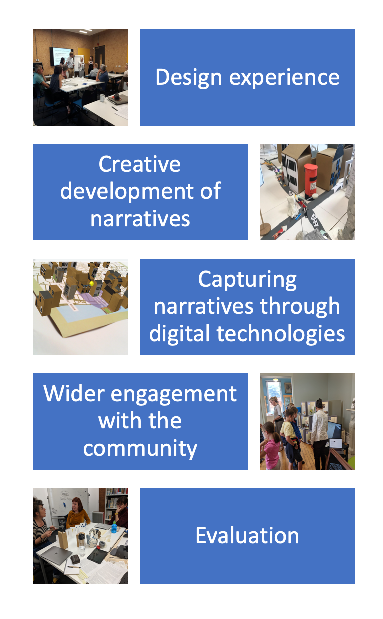
\includegraphics[width=0.3\linewidth]{images/method}
\caption{Methodology for engaging with communities as deployed by the research}
\label{fig:method}
\end{figure}

% \begin{figure}[b]
%   \centering
% 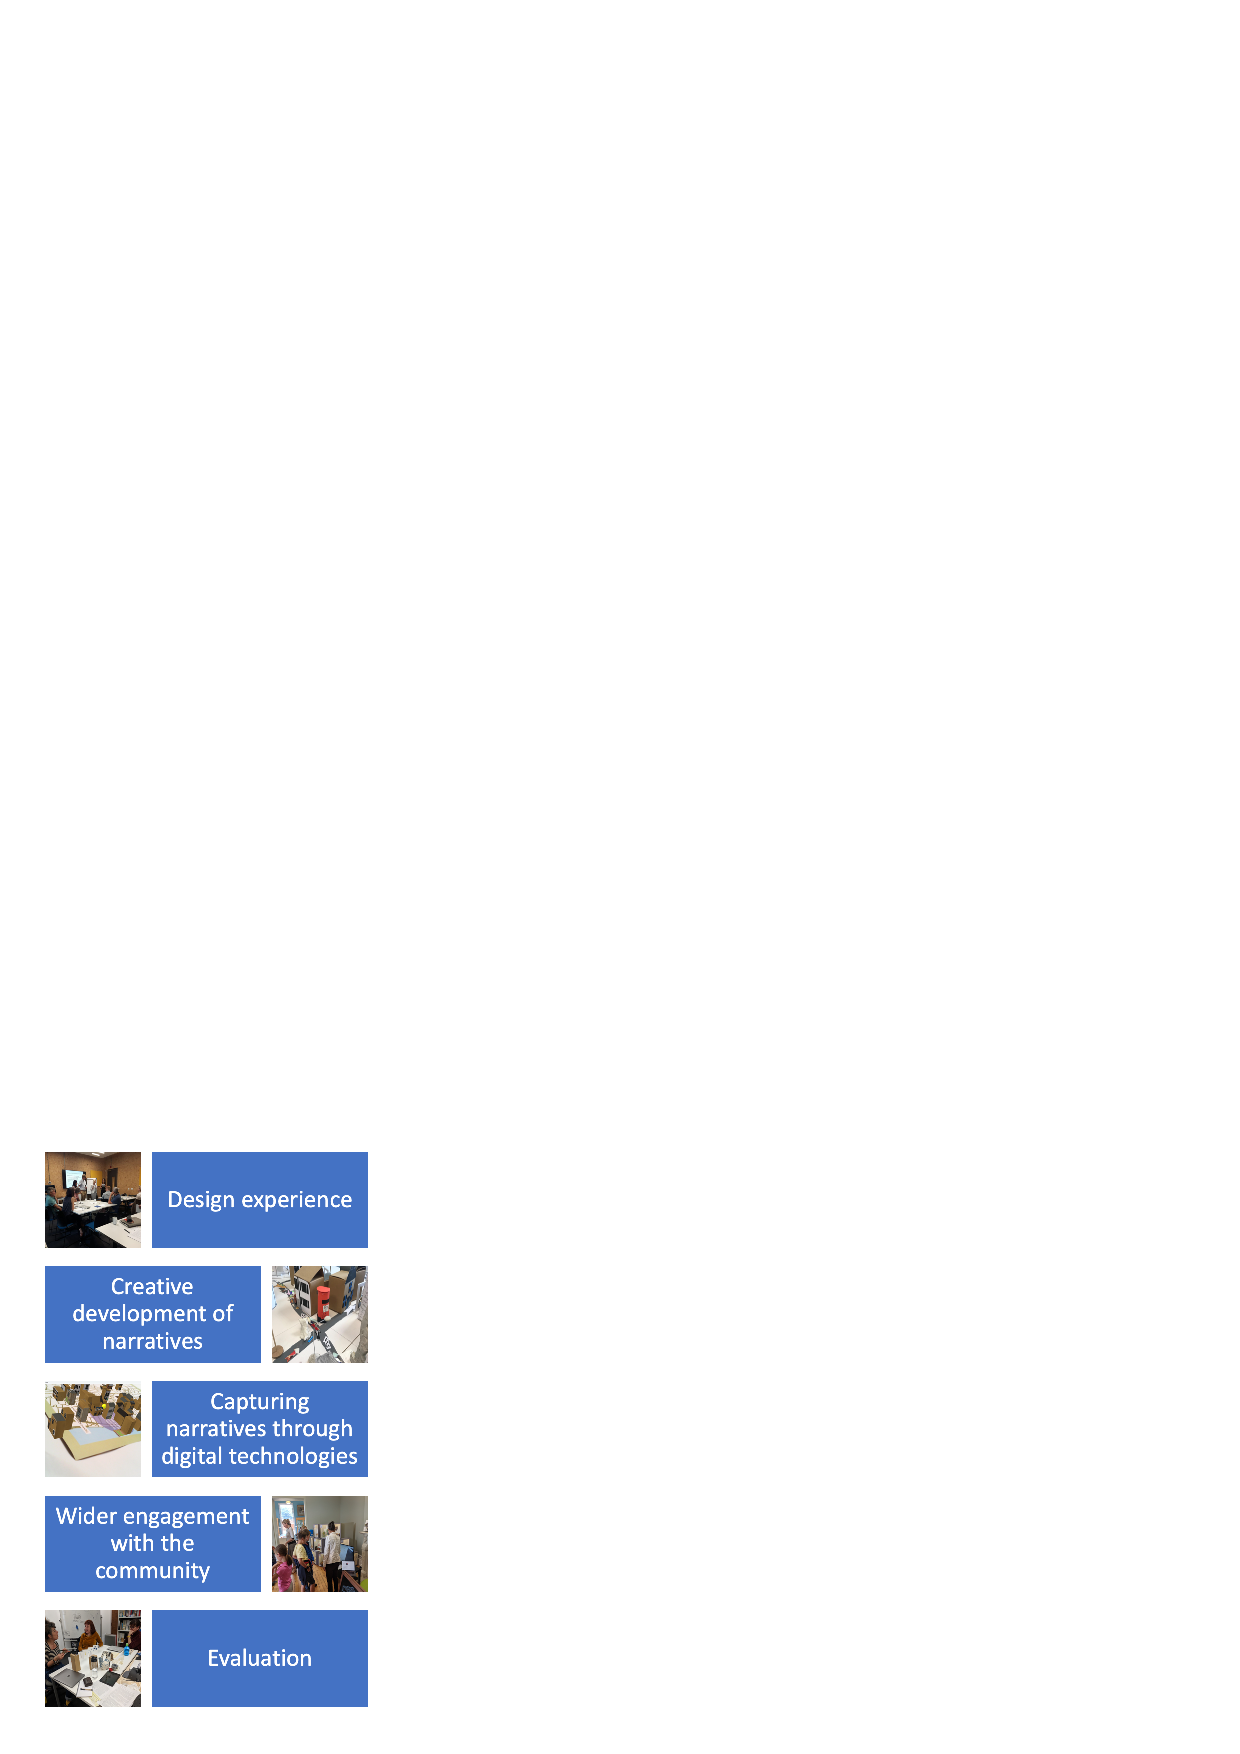
\includegraphics[width=0.8\linewidth]{images/method.png}
% \caption{Methodology for engaging with communities deployed by the research}
% \label{fig:method} 
% \end{figure}

During the design of the experiential framework, the team aimed to understand how children
could engage with their cultural environment while taking into account the 
curriculum, stimulating their creativity and addressing their well-being
needs. Attention was placed on identifying any particular issues
concerning the children who were involved in the experience, including any
educational or well-being issues affecting them at that point
in time. These issues are context dependent and are likely to be influenced by
external factors including community cohesion, socio-economic situation and
pressures from friends and family.

Thereafter, an artist facilitated ten workshops at the pilot school in order to
enable children to create narratives. These workshops used creative methods
and psycho-geography techniques to explore the journeys children make from home
to school five days a week. Psycho-geography refers to the study of the effects
of the geographical environment on the emotions and behaviours of individuals
\cite{coverley2006psychogeography}. 

The focus on the daily home-school journey was chosen due to the fact that
these journeys are a practical everyday routine. It is common that people
don't pay much attention to the places, objects and details they pass along
the route. As such, the workshops facilitated the exploration of a series of
questions:

\begin{itemize} 
  \item How do the children feel about travelling the same route five days a week, every week?   
  \item How much are children aware of the physical environment around them on these journeys? 
  \item Where do children look at when they walk? 
  \item What do children daydream about? 
\end{itemize}

As a result, children were encouraged to look up, down and all around their
local environment. They were encouraged to try to look at the streets where
they walk in a different way. In doing so, children became historians,
journalists, archaeologists in reverse, creative observers of everyday life.
Narratives, both of the children's personal lives and of elements in the
geographical landscape, were created as a result of this process. These
\emph{place-based narratives} used a mixture of physical, visual and textual
material. 

At this stage, there was no involvement of digital technologies, as it was
decided children could explore more freely their environment without the
mediation of a digital device. Instead, we used crafted elements that represented 
the narratives around the journeys children undertake from home to school. 
In order to provide a starting point, we used the concept of \emph{home}. Thus, each child produced a decorated box
which represented their house as illustrated by Figure~\ref{fig:boxes}. This
was the first observation task that enabled children -many of them for the first time-
to really pay attention to the fa\c{c}ade of their houses. 


Box-houses were used both
as geographical markers and containers of additional elements of the child's personal narrative. 
There were no
limitations on what material children could use to capture their narratives of their own journeys.
As a result, crafted elements were created from a mixture of materials such as
clay, cardboard, foam, plastic, wire, foliage, feathers.
Figure~\ref{fig:artwork}-left illustrates a mixture of the crafted materials. Children also produced drawings or collages using a
mixture of materials (e.g. foliage, printed images), illustrating their
journeys (see example Figure~\ref{fig:drawingmaps}). Some children wrote
textual content with stories of people, objects, sites and historical events they
researched on.

Finally, all elements were organised according to their geographical location
on a physical 3D map. This crafted artwork piece celebrates the individual
interpretative narratives and the collective journeys made by the children, all
converging at the shared community of school (see Figure~\ref{fig:artwork}). 

\begin{figure}[ht] \centering
\includegraphics[width=0.7\linewidth]{images/variousassets.jpg}
\caption{Crafted objects produced during the workshops documenting place-based
narratives} \label{fig:artwork} 
\end{figure}

The next steps in the methodology are explained in the following sections.

% \textbf{\begin{figure}[ht] % %     \centering % %    
% \includegraphics[width=\linewidth]{images/IMG_7377.jpeg} % %     
% \caption{Children with artwork documenting place-based narratives of central
% Hove} 
% \label{fig:childart} 
% \end{figure}} %
%-------------------------------------------------------------------------
\section{Digitisation of artwork} 
\label{dig} 
Usually, the
outcomes of psycho-geography and participatory approaches, which are not
mediated by technologies, are lost shortly after the process of engaging with
communities. The reason is that, as demonstrated by the resulting crafted
objects (Figure~\ref{fig:artwork}), while the materials which are used  are
amenable to creative approaches they are not necessarily easy for
digitisation. Hence, results from these participatory approaches are normally
disposed of shortly after their display and are rarely disseminated to
 a larger audience in their original form. 

This research explored the role of graphics technologies for i) the
digitisation of the narratives produced in order to support their
documentation and preservation; and ii) re-telling or sharing these narratives with others.
Further audiences include other members of the same micro or macro community, audiences who are
new to the geographical area and other stakeholders who might have an interest
in better understanding which elements of the cultural landscape are
significant to the community.

Several considerations were taken into  account in order to digitise the
physical artwork using 3D technologies. Decisions were mostly driven by
the fact that the process should be scalable to deal with a large amount of
crafted elements, and the crafted material was going to be rendered
as augmented content on the map. Hence, important requirements were: to
design workflows that provided craft work from every child; to produce
high-quality content; and to enable the production of good quality
representations while keeping high framerates. This meant that
the box-houses and their content were prioritised for digitisation
amongst other crafted elements. Other crafted objects, such as those
containing foliage, feathers and wire, were deemed too challenging  for
their inclusion in the AR experience during the first iterations of the
project.

% Hence, we prioritiised 3D models of the box-houses as well as to
% digitise all content inside the boxes.
% A mixed approach was used to create the 3D models of the houses. 
Two methods with suitable results for digitising this type of visual content were trialed. For both methods we used a mirrorless Sony a7R III camera with a Sigma 1:1.4 DG
macro lens. The box-houses were placed on a 360 electronic turntable, with two
Elinchrom 1000 ELC Pro HD lights with Elinchrom Rotalux softboxes used to
provide diffuse lighting. This setup ensured that the process had some degree of automation while providing
high quality results.

Afterwards, we produced 3D models both by non-image 3D modelling and image-based 3D modelling, also known as Structure from Motion (SfM). The latter process was deemed to be the most suitable for large-scale digitisation in a way which maintains the visual quality of the narrative forms. Both methods will be explained in the following subsections.

\subsection{Digitisation by 3D modelling}
Given the fact that all crafted objects are based on a physical box
which can be represented by a cuboid (see Figure~\ref{fig:boxes}), the use of
3D scanning or photogrammetry was discarded in favour of 3D modelling the
boxes using the modelling tool Blender\cite{blender}. 


\begin{figure}[ht] \centering
\includegraphics[width=0.7\linewidth]{images/boxes.png} \caption{Example
of physical model houses crafted by children depicting their own houses}
\label{fig:boxes} \end{figure}

In Blender, simple primitives, such as cubes and planes, were used
to create the shape of each box-house. The geometry began as
a simple cube, with additions such as balconies, porches or roofs being
created through the addition of planes.


The textures for each box-house were added from images taken with the digital
camera. The number of photos required for each box-house depended on its complexity. Some required only one image (of the fa\c{c}ade) with a simple
 cardboard texture used for all other faces, while others needed up to four
 (one for each side). Many of the box-houses required additional images due to
 features such as roofs or gutters. The images were taken at an angle
 perpendicular to each face in order to avoid any perspective effect. 

%  \begin{figure}[ht] \centering
% \includegraphics[width=0.49\linewidth]{images/za_tex_template.png}
% \includegraphics[width=0.49\linewidth]{images/za_tex.jpg}
% \caption{Example of unwrapped texture of house} \label{fig:pattern}
% \end{figure}


The next step was to create the
texture for each 3D model. This was done using a texture blueprint for each box-house and fitting cropped images from each side of the box. The resulting
textures were then imported into Blender. The 3D models were UV Unwrapped and
aligned with the texture. The final 3D model of a house is shown in
Figure~\ref{fig:3Dhouse}. 

\begin{figure}[ht] \centering
\includegraphics[width=\linewidth]{images/models.PNG} \caption{3D model
of house with and without texture} \label{fig:3Dhouse} 
\end{figure}

A further modelling task was to produce an animation for each 3D model. This
animation simulates the box-house roof opening and closing in a similar way people use to open and close the physical box. This takes advantage of the simplicity of the modelling approach and enables to create interesting effects during the AR experience.

The animation was implemented using
keyframes and transformations on the roof sub-objects, and each animation
lasts for 60 frames. Four animations were modelled which correspond to the
four different states a box-house can be in: 

\begin{itemize} 
  \item \textbf{Open:}
The roof has been rotated 180 degrees by its base, exposing the inside of the
box. 
\item \textbf{Opening:} Transition animation interpolated between open
and closed. 
\item \textbf{Close:} The initial state.  
\item \textbf{Closing:} Transition animation interpolated between closed and open. 

\end{itemize}


% The drawings and other written content inside the boxes were scanned using a
% flat-bed scanner. Figure \ref{fig:drawingmaps} shows examples of this digital
% content. Further editing was done to the images in order to blur personal
% information, for example names and addresses. The images were applied as
% textures to 3D planes so that they can be visualised as a 3D model.

% \begin{figure}[ht] \centering
% \includegraphics[width=0.6\linewidth]{images/lkp1.jpg}
% \includegraphics[width=0.6\linewidth]{images/mgp2.jpg}
% \includegraphics[width=0.6\linewidth]{images/fhp1.jpg} 
% \caption{Drawings
% of children detailing local geographies, journeys from home to school and
% objects in the environment.} \label{fig:drawingmaps} 
% \end{figure}

% Moreover, objects crafted in clay were 3D scanned using the Artec3D handheld
% 3D scanner. Additional 3D models were accessed from a relevant project
% \cite{14f05b94a1844f5e850c87fc9d042c59}. This project undertook the
% digitisation of public sculptures in the same geographical area using a
% crowdsourcing approach and published the resulting 3D content on the web.


\subsection{Digitisation by image-based 3D modelling}
In order to deal with a potentially large amount of crafted items, we
also experimented with a semi-automated image-based workflow. The main
motivation behind this is that it allows us to process a wider variety
of shapes, without having to deal with modelling every customised crafted item. The main challenge, that we had to address here, was to ensure the visual quality of the items by capturing both the
shape and the colour accurately. 


As mentioned before, all box-houses were created using a similar cardboard box as a starting
point. Then each house was customised using coloured paper and crayons.
Although the areas coloured with crayons displayed some shine when catching
beams of light, most material was fairly non-reflective. To ensure colour fidelity of the
artefacts, we followed a similar method to \cite{Gaiani_2017}. This ensured that the 3D models which resulted from the process had a good and uniform quality, particularly with regards to the cardboard
textures.


For the colour characterization in the lighting environment in which we performed the
digitisation, we made use of the X-Rite ColorChecker. The X-Rite ColorChecker automatically detects the
colour checker and produces an ICC profile which is then applied to all
images.


Thereafter, the workflow required of an operator taking a set of images
using the automated setup. For this, each box-house was placed on a
turntable with a white background and photographed every $20\degree$
over three full $360\degree$ rotations. For each rotation, the camera is
rotated $90\degree$, generating in total between 54 - 60 images. During the photogrammetric acquisition, we also made use of a measuring bar with circular cross-type targets. This
allows to introduce scale to the 3D model when it is later processed.

The digital images were shot using ISO 100, and an aperture of F/11. The
images were shot in RAW and later processed using the ICC profile before
exporting them as JPEGs to be used during the image-based 3D modelling. The sets of images were then automatically processed by a Python
script employing the Agisoft Metashape API \cite{Metashapesite}. This
script reads the images from a folder, processes a 3D model, detects the
targets captured in the image, scales and centres the model as shown in
Figure \ref{fig:metashape}. All these steps are fully automated.


\begin{figure}[ht] \centering
\includegraphics[width=1\linewidth]{images/metashape.png} 
\caption{3D model of a box-house generated through a photogrammetry automated
process} \label{fig:metashape}  
\end{figure}


Next, a manual process was required to remove the excess geometry,
including the measuring bar. Finally, the resulting 3D model was
decimated to a size of 5,000 triangles and a texture with a reduced
resolution. All content had to be post-processed in order to make it
web-ready for the AR experience. This required developing workflows for
the production of suitable 3D meshes (in terms of size/quality) for
distribution over the web.  % Moreover, the textures had to be
Textures were also optimised for web delivery as the initial images had % produced with
very high resolution and large file size. This was done by deploying % them
the ImageOptim web service \cite{ImageOptim}.   %Furthermore,
All images were resized to dimensions which are powers of two
% (e.g. % 2048x2048, 512x1024)
to facilitate loading. 
% The images produced
%used a final % resolution of 96dpi. For this, the 
The glTF file format was used to encode the 3D models and their animation for the AR
experience. The glTF (GL Transmission Format) is a common specification for
the efficient transmission and loading of 3D scenes and models,
especially by web applications \cite{khronos}. This format reduces both the size
of 3D resources and the execution processing required to decompress and
use them. It stores a full scene description in JSON format, which
includes node hierarchy, cameras, and materials and it also contains
descriptor information about animations and meshes.


\subsection{Measuring colour fidelity} Ensuring and measuring colour
fidelity of 3D models in an image-based 3D modelling process is still an
open research matter. As such, we designed a method to evaluate the
resulting colour fidelity of the 3D models produced by the
digitisation phase. For this, we made the assumption that all areas of
the 3D model displaying a cardboard texture would have very similar
colours.

Our method deploys small patches (80 by 80 pixels) extracted from
textures of two different 3D models, as shown in Figure
\ref{fig:texturepatches}. For this, we selected areas that correspond to the
non-decorated areas of the cardboard boxes, assuming that these two areas
must be similar in colour. 


To understand the perceived differences between colours from the two different textures, we utilised the $\Delta$E (Delta E) measurement. $\Delta$EE is a metric for understanding how the human eye perceives
colour difference, which was proposed by the International Commission on
Illumination (CIE). On a typical scale, the Delta E value will range
from 0 to 100. The difference of less than 1.0 between two colours means
that the difference is not perceptible by human eyes. Any values above
11 indicate colours are more similar than opposite, while a value of 100
means that colours are the exact opposite. We hypothesised that getting
values between 1-10 meant the changes in texture colour would only be
perceptible through close observation or at a glance in the worst
case scenario.

In order to calculate this metric, we firstly had to select the best
colours in the texture patch to compare. For this, we looked for the
dominant colours on a given patch using K-means cluster analysis. By
using this method, we produced a distribution of the five (5) most dominant
colours as illustrated in Figure \ref{fig:distribution}. We then tested
the most dominant colours against the most dominant colours of the other
texture.


\begin{figure}[ht] \centering
\subcaptionbox{Two 80 x 80 pixel texture patches from different 3D models\label{fig:textures}\linebreak}
  {\includegraphics[width=0.45\linewidth]{images/m1tex_80x80.png}
   \includegraphics[width=0.45\linewidth]{images/m2tex_80x80.png}
  }\\[-0.5\baselineskip]
  \subcaptionbox{Five most dominant colours on the texture and percentage distribution\label{fig:distribution}}
  {\includegraphics[width=0.45\linewidth]{images/domtex1.png}
   \includegraphics[width=0.45\linewidth]{images/domtex2.png}
  }\\[-0.5\baselineskip]

 \caption{Texture patches used to evaluate the quality of colour fidelity across different 3D models resulting from the image-based 3D modelling process} 
 \label{fig:texturepatches} 
\end{figure} 


To calculate $\Delta$E for the colour in the texture patches, we firstly took 
the top five (5) most dominant colours of a texture
patch and converted them to the CIELAB colour space. CIELAB colour space,
also known as CIE L*a*b*, is the colour space defined by the International Commission on Illumination (CIE) in 1976. The colour space allows to express colour as
three values: lightness, a* from green to red, and b* from blue to yellow. After 
representing colour in the CIELAB space, we then applied the 
CIELAB 2000 $\Delta$E algorithm using Python colormath library. 

Table \ref{tab:delta} presents a comparison across the five (5) most dominant colours for textures $ A $ and $ B $. 
%Beside
All colours present a similarity of under 3.5, meaning there is only a perceptible difference amongst the textures when very closely inspected. It should also be noted that, when comparing a colour to another colour with a similar percentile, they are very similar in their $\Delta$E value. 

\begin{table}[h]
\begin{tabular}{ | l | c | c | c | c | c |}
\toprule
  & $ A_0 $ (38.94\%)  & $ A_1 $ (28.66\%) & $ A_2 $ (18.78\%)& $ A_3 $ (8.05\%) & $ A_4 $ (5.58\%)  \\ 
\midrule
 $ B_0 $ (34.00\%) & \textbf{1.528} & 2.092 & 0.944 & 2.719 & 0.266  \\ 
 $ B_1 $ (28.42\%)& 0.959 & \textbf{1.515} & 0.427 & 2.145 & 0.478  \\ 
 $ B_2 $ (19.84\%)& 2.121 & 2.685 & \textbf{1.531} & 3.31 &  0.806 \\ 
 $ B_3 $ (10.89\%) & 0.403 & 0.893 & 0.458 & \textbf{1.514} & 1.104  \\ 
 $ B_4 $ (6.84\%) & 2.845 & 3.408 & 2.254 & 4.032 & \textbf{1.528}  \\ 
\bottomrule
\end{tabular}
\caption{$\Delta$E value comparison for the top five colour values for each texture patch}
\label{tab:delta} 
\end{table}

The evaluation results demonstrate that our method for generating 
low resolution textures for the 3D models produces good and uniform quality 
in terms of colour. This allows to
follow a standardised process which can be deployed for large-scale
content, while ensuring the visual quality of the outcomes.


\section{Augmented Reality (AR) Map Development} \label{tech} 

While the process for digitisation is better understood by the research
community in terms of deciding which technologies are more appropriate for certain artefacts, the requirement to re-tell user-created narratives has not previously been fully
explored. Thus, there are many potential digital experiences which could be
deployed for this purpose. 

Here, we propose a novel approach for re-telling users' narratives. This approach
combines both physical and digital elements of a CH experience. The digital element
is intended to serve as a canvas for users to interact with the journeys and
find more information about the narratives through hyperlinks. 

From early on in the research, it was clear that communicating the
geographical location was critical to re-telling the narratives. However,
using precise geographical information, such as in a Geographical Information
System (GIS), was not possible without having to reveal the exact address of the members of the community. Hence, the idea of providing the
content geographically in-situ was discarded. Instead, the research
incorporated a means which is very familiar to people when visiting a new
location. This is the communication of specific information through a printed
map (e.g. a tourist map or a building map). Printed maps allow the
abstraction of geographical/spatial information while enabling the reader to
orient themselves in space. Augmented Reality (AR) is then used to embed
the digitised narratives without losing their geographical information. AR has also the advantage that multiple interpretations can be simultaneously embedded into the same visual information. 

Furthermore, the research considered the need to create physical media which is
cost-effective to produce and distribute to a large audience. As such, all
the physical elements of the experience can be easily reproduced by the user by
printing a PDF map. Also, the digital element is easily accessible from a
web browser on a PC, tablet or smartphone so that there is no need to install an application. 

The Augmented Reality web-application renders a 3D scene with the crafted
houses, which are positioned over the printed map in a similar way to the
crafted artwork (see Figure~\ref{fig:ARexperience}). When the user clicks or
taps on each of the houses, an animation is triggered to simulate the box
being opened. The content inside the box is then rendered on a viewer for the
user to inspect the elements of narratives in more detail. 

The following sub-sections will describe in detail how the different
components of the Augmented Reality (AR) map were developed.

\subsection{Development of printed graphical map} %talk about the development
% process for the printed map: mapnik, openstreetmap data, rendering of scene, 
The development of the printed map addressed various requirements as described
below:

\begin{itemize} 
  \item The map should display information on the street layout in a way which is easily understood by the user. 
  \item The map should not reveal the precise geographical location of the houses. 
  \item The map should be self-contained in terms of telling the user how to access 
  the digital element of the experience. 
  \item The map should include a marker for the Augmented Reality which is not too distracting. 
\end{itemize}

In order to address the first two requirements, a customised rendering of a
map was created. This map displayed information, which is geographically
accurate, but detailed information, such as street names, was omitted. The
open-source mapping toolkit Mapnik \cite{mapnik} was used to generate the map.
This toolkit, with binding in Python, can programmatically generate rendering
of geographical maps with the appearance the user wants. For this, an XML
stylesheet is created filtering only the information about the streets for
rendering, while providing other information, such as colour and line thickness.
Thereafter, a Python script processed this stylesheet to produce the final
rendering. Geographical data of Brighton and Hove (UK) was retrieved from OpenStreetMap
\cite{OpenStreetMap} in the OSM data format. This data was then used as input
to the script in order to produce the rendering of the map in PNG format (see
Figure~\ref{fig:map}).


\begin{figure}[b]
\includegraphics[width=\linewidth]{images/maprender.jpg}
\caption{Rendering of map using the Mapnik toolkit} \label{fig:map} 
\end{figure}
 
The rendering of the map was further processed in the GIMP image processing
tool \cite{gimp} in order to include the names of relevant
geographical references as additional information. All references were extracted from the children's
narratives and included historic buildings, libraries, museums, parks,
a cemetery and sculptures. Instructions on how to access the website with the AR
experience were also included.

Furthermore, a fiducial code or marker with the logo of the school was
included as illustrated in Figure~\ref{fig:print}. The marker serves both as a
way to identify the geographical location of the school as well as to enable
the AR content. Other marker-less solutions were considered. However, AR over
the web does not have yet the performance required for marker-less AR, which
is normally distributed via apps and is often reliant on Google's ARCore
software. Hence, not wanting to compromise the web-based delivery, the
logo-based marker was considered a suitable solution.


Finally, general information about the project was included as a
double-sided page (see Figure~\ref{fig:print}). In this way, the print out of the double-sided
page is a self-contained output of the project.

% The following subsection will describe how the 3D scene which is augmented
% on the map was developed.



% The following section will describe the implementation details of the AR
% application.

\subsection{Web based Augmented Reality (AR)} % %talk about how it was put all

In order to make the AR maps easily
accessible, the research makes use of an \emph{Immersive Web} approach, which
refers to virtual world experiences hosted through a browser, covering both
Virtual Reality and Augmented Reality experiences developed for AR-enabled
devices \cite{imweb}. The WebXR API is currently the experimental
specification for both augmented reality and virtual reality devices
\cite{webxr}.

Nowadays, web-based AR technologies make use of APIs, such as the WebRTC and WebVR
to enable the delivery of AR through a web browser. Other available frameworks include Argon.js \cite{Argon.js}, AR.js based on A-Frame
\cite{aframe}, Awe.js, \cite{Awe.js}, 8th Wall \cite{8th}. All these
frameworks make use of Javascript and some of them offer marker-less
capabilities (e.g. 8th Wall) through a paid service.

Although AR installed as an application on a mobile device often offers better
performance, it was deemed that a web-based approach would enable more people
to access the experience from a diverse set of devices and platforms. For
instance, frameworks such as Vuforia \cite{Vuforia} are not web based and
require payment in order to remove watermarks. 
% %However, they are
% markerless and offer high stability and many extra features. Nevertheless,
% they require to be installed as an app and the heritage sector is increasingly
% reluctant to use this approach.

Ar.js and A-Frame were used as a framework to develop the web-based experience
as they are both open-source. A-Frame is an open-source web framework for
building both Virtual Reality (VR) and Augmented Reality (AR) experiences
based on Three.js. A-Frame is an entity component system framework, allowing to create 3D scenes using HTML and Javascript. Most 3D operations are
performed by A-Frame in memory with minimal overhead and are rendered with
WebGL \cite{webgl}, which binds to OpenGL or Direct3D. A-Frame is meant to
give suitable latency and framerate with browsers, such as Firefox with WebVR.


\begin{figure}[ht] \centering
\includegraphics[width=0.48\linewidth]{images/ARcontentw_sculpture.png}
\includegraphics[width=0.48\linewidth]{images/animationARexperience_zoom.png}
\caption{AR Map experience showing the different house models and a sculpture in the geographical area (left); animation to open the house is triggered when the user taps on a house model revealing a visualisation
 of the child's map (right)} \label{fig:ARexperience}
\end{figure}
 
In the project, the Aframe raycaster is used, which is built
on the Three.js raycaster. On collision with an object, the raycaster triggers
an event on said object. 

The AR.js API is employed to render all elements of the scene, including the
houses and other additional 3D content. The marker on the printed map is used
to position the 3D scene on the printed map (see
Figure~\ref{fig:ARexperience}-top). In order to enable user interaction with
the 3D models, the Three.js raycaster is deployed. The system triggers a different
behaviour according to the type of object that is clicked: 

\begin{itemize}
\item When the user taps on a house, the animation to open or close the house
is triggered (see Figure~\ref{fig:ARexperience}-bottom). After playing the
animation, the content which belongs to each box is displayed on the Universal
Viewer \cite{uv}. The implementation includes the capability to add hyperlinks
to direct the user to explore further information on the web. 
\item When the
user taps on a 3D model of a sculpture, the object acts as a hyperlink to
relevant information, which has been curated by a researcher.  
\end{itemize}

% At this point, the desire to give more details on the children's maps gave
% us the idea of adding an information button that would allow us to access
% this supplement. The first step was to add a url to the index.html file for
% homes that needed more information.  Then, in the viewer.html file, a button
% was added after the close button (which allows you to return to the home
% page).  The next step was to add an event listener to this button to give it
% a function. This function was to open a new window with a url. And finally,
% when the house did not require any further information, the button should
% not be visible to the user. What has been managed by defining a classList
% equal to "hide" at the button

The framerates and latency achieved with the current development were tested
in various platforms (see Table \ref{table:framerates}). Latency is an
expression of how much time it takes for a packet of data to get from one
designated point to another. As expected, the framerates vary with the
processing power and graphics card capabilities. The highest framerate
achieved is of 60 frames per second (fps) on a mobile phone (see row 2 in
Table~\ref{table:framerates}). However, the responsiveness on a mobile phone for
racytracing performed worse on the mobile device than on a laptop or PC.

High framerate and low latency is the ideal and these seem to have a direct
correlation to the CPU/GPU for mobile devices. 60fps/16ping seems to be the
best across all devices. Nevertheless, the fact that a Google Pixel 2 and 3 both
have the same, despite differences in CPU/GPU, suggests that improvements are minor
for newer mobile phone models. The lower framerate shown by a MacBookPro
and an ASUS Zenbook indicate that the APIs are well optimised for mobile
architectures.

%One possible reason for this could be due to the framerate of the camera
%(newer phones have a high quality, high framerate camera which is better than
%laptop webcams or tablets).

% \begin{table}[h] \centering 
% \begin{tabular}{|p{90px}|c|c|} \hline Device & 
% Framerate (fps) & Latency (ping)\\  \hline \hline 
% Google Pixel 3 (Octa-Core,
% Adreno 630 1 MB, 4 GB LPDDR4X) &  60 & 16\\ \hline
%  Google Pixel 2 (Octa-core,
% Adreno 540 1 MB, 4 GB LPDDR4X)  &  60 & 16\\ \hline
% Pocophone F1 (Octa-Core, Adreno 630, 6 GB) & 60 & 16 \\ \hline 
% MacBook Pro
% (Intel Core i9, Radeon Pro Vega 20 4 GB, 32 GB DDR4, 720p camera - 30 fps)  &
% 50 & 17\\ \hline 
% Nexus 5X (Hexa-Core, Adreno 418 512 KB, 2 GB LPDDR3) & 32 &
% 42 \\ \hline  
% Nexus 5X (Hexa-Core, Adreno 418 512 KB, 2 GB LPDDR3) & 32 & 42
% \\ \hline 
% ASUS ZenBook UX330UA (Intel(R) Core(TM) i5-7200U CPU, RAM 8 Go) & 30
% & 20\\ \hline 
% Galaxy Tab S3 (Quad-core, Adreno 530, 4GB of RAM) & 18 & 50\\
% \hline \end{tabular} 
% \caption{Testing web-based AR application in various
% devices of scene containing 1,176 triangles} \label{table:framerates} 
% \end{table}


% \subsection{Link to additional information on objects}


%-------------------------------------------------------------------------
\section{Preliminary evaluation} \label{eval} An evaluation took place before
the start of the project in order to provide a baseline to measure the
project outcomes. During this survey, children were asked about their
well-being, confidence and overall resilience in life. Another evaluation took
place after the school workshops. The collected feedback showed that the proposed creative process made children feel better about themselves and improved their overall mood. For
instance, there was a 45\% increase in children reporting feeling very happy,
18\% increase in children reporting liking themselves, a 15\% increase in
children reporting that they coped with difficult situations happily or very
happily, and a 15\% increase in children feeling liked by other people. During
this evaluation, the AR Maps were not evaluated as these had not been developed yet.

In July 2019, a ``celebration'' of the artwork and the children's journeys took
place at the Hove museum (UK). On this day, all children were invited to
bring their families and friends to the museum to show them their artwork and talk to the
researchers who developed the AR application. The setup in the museum included
three areas: 1) an area to display the artwork and engage with the AR
experience (see Figure \ref{fig:museum}-left), 2) an area where the visitors could engage with the creative process and create their own journeys (see Figure
\ref{fig:museum}-right), and 3) an area for visitors to experience a creative
application in Virtual Reality. It was considered that this provided a good mixture
of hands-on and creative digital activities to engage visitors.

On the ``celebration'' day, families and friends saw the artwork for the first time. That day was also the first time the children experienced the AR Map. Hence, a
large amount maps were printed in 80 gsm recycled paper and distributed amongst the
visitors of the museum, while extra copies were sent to school.

\begin{figure}[ht] \centering
\includegraphics[width=0.48\linewidth]{images/IMG_20190720_103105.jpg}
\includegraphics[width=0.48\linewidth]{images/IMG_20190720_151644.jpg}
\caption{Setup at the Hove museum for the celebration of the artwork and
release of the AR application and area with the original map (left); area
where people could engage with the creative process (right)} \label{fig:museum}
\end{figure}
 
Initial feedback from the children provided evidence that the experience was
particularly engaging because of the Augmented Reality aspect. Children were keen to test
the printed map on their or their carers' phones and were eagerly looking for their house and their stories on the map.
Most children were very proud to see the content they had produced being
rendered on the screen, after touching on their house. Moreover, they were happy to tell
others about their narratives and share information about the journeys they make every day. Others, who had no
direct connection to the children, found the AR experience very interesting too.
hence, they would randomly tap on houses and inspect the content that children had created.
 
 During the testing, we also noticed some technical issues with respect to the AR aspect. The
 most common amongst these were related to the size of the screen to experience a large
 amount of visual content, as well as the responsiveness of smart devices with less
 powerful CPU/GPU. Despite the cross-compatibility of the AR framework, there
 were also issues with iOS devices including iPhones and iPads. Furthermore,
 the testing made evident that clearer instructions on the printed map
 were needed. Some people would immediately switch their cameras on (without
 going first to the website) and be surprised that there was no displayed content. All this feedback is currently being incorporated into a second release of the AR Map experience. 


%-------------------------------------------------------------------------
\section{Conclusions} \label{conc} This paper presented novel research for the
development of approaches and technologies enabling communities to
meaningfully engage with their cultural environment in creative ways. Thus,
the paper described the methodology for deploying the proposed approach which was then tested
with a local community in Brighton and Hove (UK). As a result, children
engaged in a process which included the exploration of their community; the conception of narratives evidencing their daily journeys from home to school; the production of these narratives by using creative means; and the experience and sharing of these narratives through the AR map with members of their communities and beyond.

The paper demonstrated how mobile and augmented reality technologies provide a
novel element for re-telling communities' narratives to wider audiences. These
experiences combine physical maps, such as those widely used for tourists,
with augmented 3D using Immersive Web technology. 

Feedback from users demonstrates the potential of these approaches to raise
awareness about the cultural elements of the areas where communities live. Moreover, the proposed framework can positively affect participants, in this instance children, while enhancing their sense of belonging, well-being and happiness. Particularly, the AR elements seem to have triggered the curiosity of users to explore different narratives, while becoming aware about other people's viewpoints with regards to their local environment.

Future work for the research involves the usability evaluation of the Augmented Reality aspect
in order to understand how to overcome issues such as latency and
user-friendly access to the content when this is viewed from a mobile device.
Another area to explore is how to ease the digitisation of the material which is difficult to capture; especially crafted objects which are made of feathers, wire and generally objects that present certain complexities. Children could also
become involved in the digitisation process. This not only would enhance their digital
skills, but would also support the emergence of new links between the crafted materials and
CH content that could be curated by heritage experts. 

%type of experiences can allow community members to experience narratives
%relating to people, objects, sites and events which are of importance to the
%communities that live amongst them.


Ultimately, the research contributes towards enabling communities to
participate in the identification, preservation and dissemination of cultural heritage content. Such active community involvement contributes towards the democratisation of CH, while supporting at the same time the emergence, exploration and understanding of the multiple and diverse meanings of heritage information.


\section{Acknowledgements} We would like to thank Bec Britain and Jo Coles
from Our Future City who co-designed, developed and delivered the workshops, as
well as Peter Chivers for supporting the activity. We also thank Karin Janzon,
from Hove Civic Society, for her continuous support in engaging communities in
Hove, as well as Kate Howland who contributed to ideas for the community engagement. 
Finally, we would like to acknowledge the teachers and children of the
school in Hove for participating with so much enthusiasm in the research. 
The project has received support from the Santander Undergraduate Research Scheme
at the University of Brighton.

% \balance



%\bibliographystyle{eg-alpha}
\bibliographystyle{ACM-Reference-Format}
\bibliography{egbibsample} 

% \newpage \begin{figure*}[ht] \centering
% \includegraphics[width=0.49\linewidth]{images/side.png}
% \includegraphics[width=0.49\linewidth]{images/side1_cropped.png}
% \caption{Printed graphic for AR experience containing: left) rendered map by
% mapnik, AR pattern and instructions for access, and right) general information
% about the project} \label{fig:print} \end{figure*}



\end{document}
